% Этот шаблон документа разработан в 2017 году
% Владимиром Коротковым (kvamob@mail.ru) 
% для подготовки и печати паспортов скважин 

\documentclass[a4paper,12pt]{article} % добавить leqno в [] для нумерации слева

%%% Работа с русским языком
\usepackage{cmap}					% поиск в PDF
\usepackage{mathtext} 				% русские буквы в формулах
\usepackage[T2A]{fontenc}			% кодировка
\usepackage[utf8]{inputenc}			% кодировка исходного текста
\usepackage[english,russian]{babel}	% локализация и переносы

%%% 
\usepackage{rotating}				% Поворот текста
\usepackage{multirow}				% Таблицы с объединенными ячейками

%%% Дополнительная работа с математикой
\usepackage{amsmath,amsfonts,amssymb,amsthm,mathtools} % AMS
\usepackage{icomma} % "Умная" запятая: $0,2$ --- число, $0, 2$ --- перечисление

%%% Символ диаметра
\DeclareFontEncoding{LS1}{}{}
\DeclareFontSubstitution{LS1}{stix}{m}{n}
\DeclareRobustCommand{\diameter}{%
	\text{\usefont{LS1}{stixscr}{m}{n}\symbol{"60}}%
}

%% Номера формул
\mathtoolsset{showonlyrefs=true} % Показывать номера только у тех формул, на которые есть \eqref{} в  тексте.

%% Шрифты
\usepackage{euscript}	 % Шрифт Евклид
\usepackage{mathrsfs} % Красивый матшрифт

%% Свои команды
% \DeclareMathOperator{\sgn}{\mathop{sgn}}

%% Перенос знаков в формулах (по Львовскому)
% \newcommand*{\hm}[1]{#1\nobreak\discretionary{}
%	{\hbox{$\mathsurround=0pt #1$}}{}}

%%% Работа с картинками
\usepackage{graphicx}  % Для вставки рисунков
%\usepackage[export]{adjustbox}
\graphicspath{{images/}{images2/}}  % папки с картинками
\setlength\fboxsep{3pt} % Отступ рамки \fbox{} от рисунка
\setlength\fboxrule{0.2pt} % Толщина линий рамки \fbox{}
\usepackage{wrapfig} % Обтекание рисунков и таблиц текстом

%%% Работа с таблицами
\usepackage{array,tabularx,tabulary,booktabs} % Дополнительная работа с таблицами
\usepackage{longtable}  % Длинные таблицы
\usepackage{multirow} % Слияние строк в таблице

%%%%%%%%%%%%%%%%%%%%%%%%%%%%%%%%%%%%%%%%%%%%%%%%%%%%%%%%%%%%%%%%%%%%%%%%%%%%%%%%%%%%%%%%%%%%%%%%%%%%%%%%%

%%% Заголовок
\author{ООО <<Гидросфера>>}\label{company}
\title{ПАСПОРТ РАЗВЕДОЧНО-ЭКСПЛУАТАЦИОННОЙ СКВАЖИНЫ}
\date{\today}
%%%======================================================================================================
\newcommand{\txtExecutor}{ООО <<Гидросфера>>}			% Исполнитель
\newcommand{\txtYear}{2017}			% Исполнитель
\newcommand{\txtNumber}{№ 1р-э}  					% Номер скважины
\newcommand{\txtPump}{<<Напор>>}  					% Марка насоса
\newcommand{\txtAddress}{Свердловская обл, г. Екатеринбург, ул. Кутузова, дом 47} 
\newcommand{\txtHeight}{ }							% Абс. отметка устья скважины
\newcommand{\txtCadaster}{66:41:0508041:8} 			% Кадастровый номер
\newcommand{\txtCoords}{57,061755 59,504491}		% Координаты скважины
\newcommand{\txtDepth}{50,0}						% Глубина скважины
\newcommand{\txtDebit}{5,0}							% Дебит скважины
%% ../ приуроченных к ...
\newcommand{\txtGeology}{трещиноватым разностям палеозоя}
\newcommand{\txtLevel}{5,0}							% Уровень воды в скважине
%%%======================================================================================================


\begin{document} % конец преамбулы, начало документа

%% Титульная страница

\begin{titlepage}
	\begin{center}
		\textbf{\txtExecutor}
		\vspace{5.5cm}
		
		{\LARGE ПАСПОРТ РАЗВЕДОЧНО-ЭКСПЛУАТАЦИОННОЙ СКВАЖИНЫ}
		\vspace{0.25cm}
		
		\underline{для хозяйственно-бытового водоснабжения}
		
		\bigskip
		
		на участке по адресу:
				
		\underline{\txtAddress}
		
		\bigskip
		Кадастровый номер \txtCadaster
		
		\vfill
	
		\bigskip
		
	\end{center}

	\vfill
	
	\newlength{\ML}
	\settowidth{\ML}{«\underline{\hspace{0.7cm}}» \underline{\hspace{2cm}}}
	\hfill
	\begin{minipage}{1.0\textwidth}
		Директор ООО <<Гидросфера>> к.г.м.н.
		\underline{\hspace{\ML}} А.\,А.~Кашкаров\\
	\end{minipage}%
	
	\bigskip
	
	\vfill
	\begin{center}
		Екатеринбург, \txtYear
	\end{center}			

	\end{titlepage}

%%%%%%%%%%%%%%%%%%%%%%%%%%%%%%%%%%%%%%%%%%%%%%%%%%%%%%%%%%%%%%%%%%%%%%%%%%%%%%%%

	\begin{center}
		\textbf{ПАСПОРТ}

		разведочно-эксплуатационной скважины \txtNumber, cооруженной 

		\txtExecutor, г.Екатеринбург

	\end{center}


	\bigskip
	
	Адрес участка: 

	\underline{\txtAddress}

	\bigskip

%	\begin{align}
%		\text{Кадастровый номер}&: \text{\txtCadaster} \\
%		\text{Координаты скважины}&: \text{\txtCoords} \\
%		\text{Абсолютная отметка устья скважины}&: \text{\txtHeight} \\
%	\end{align}
	
	Кадастровый номер: \txtCadaster

	Координаты скважины: \txtCoords
	
	Абсолютная отметка устья скважины: \txtHeight

	\begin{figure}[h]
		\fbox{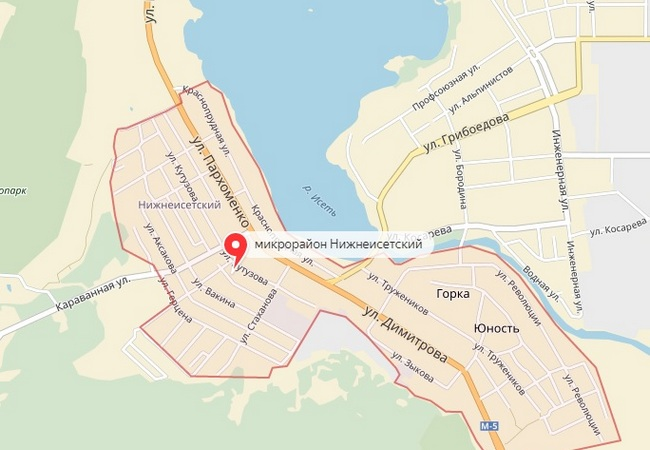
\includegraphics[width=\textwidth]{map.jpg}}
		\caption{Обзорная карта расположения скважины}
	\end{figure}

    \section*{Геолого-технические данные скважины}

    Разведочно-эксплуатационная скважина сооружена \txtExecutor. Имеет общую глубину \txtDepth \,м.   Бурение производилось вращательно-роторным способом станком УРБ-2-2А.

    \bigskip

    Бурение начато << >> \txtYear \,г. 

	Бурение окончено << >> \txtYear \,г.

	Приемно-сдаточный акт на скважину подписан << >> \txtYear \,г.
	
	\bigskip
	
	При бурении скважины пройдены следующие горные породы:
	
	\section*{Конструкция скважины}

	Высота оголовка	\underline{+0,4} м	от поверхности земли. 
	
	\bigskip

	Обсадная колонна:

	диаметром \underline{160} мм от \underline{+0,4} м до \underline{10,0}  м  		
	
	диаметром \underline{128} мм от \underline{+0,4} м до \underline{30,0} м
	
	\bigskip

	Открытый ствол:

	 диаметром \underline{132} мм от \underline{30,0} до \underline{38,0} м 
    
    \bigskip
	
	Фильтровая колонна \underline{нет}
	
	\bigskip

\begin{tabular}{|c|c|}
	\hline 
	\rule[-1ex]{0pt}{2.5ex} №№ & Конструкция: \\ 
	\rule[-1ex]{0pt}{2.5ex} п.п. & каркас, расположение отверстий, тип, сетка, проволока, диаметр и тд. \\ 
	\hline 
	\rule[-1ex]{0pt}{2.5ex} 1. & От +0,4 до 10,0 м   надфильтровая часть \diameter 160 мм полиэтиленовая труба \\ 
	\hline 
	\rule[-1ex]{0pt}{2.5ex} 2. & От +0,4 до 30,0 м   надфильтровая часть \diameter 128 мм полиэтиленовая труба \\ 
	\hline 
	\rule[-1ex]{0pt}{2.5ex} 3. & От 30,0 до 38,0 м   открытый ствол \diameter 132 мм \\ 
	\hline 
\end{tabular} 

\bigskip

Рабочая часть скважины установлена на основании литологического описания пройденных горных пород и результатов геофизического исследования скважины.

%\newpage

Конструкция и глубина сооруженной скважины приведены в следующей таблице:

\bigskip

\begin{center}
\begin{tabular}{|l|c|}
	\hline 
	Глубина в м. & \txtDepth \,м \\ 
	\hline 
	Бурение & Диаметром 165 мм \\ 
%	\hline 
	& от +0,4 до 10,0 м \\ 
%	\hline 
	& Диаметром 132 мм \\ 
%	\hline 
	& от 4,0 до 30,0 м \\ 
%	\hline 
	&  \\ 
	\hline 
	Конструкция & Бурение от 0,0 до 38,0 м \\ 
%	\hline 
	& Обсадка от +0,4 до 30,0 м \\ 
	\hline 
	Обсадка & Диаметром 160 мм \\ 
%	\hline 
	& от +0,4 до 10,0 м \\ 
%	\hline 
	& Диаметром 128 мм  \\ 
%	\hline 
	& От +0,4 до 38,0 м \\ 
	\hline 
\end{tabular} 
\end{center}

\bigskip

Произведена затрубная гидроизоляция обсадной колонны диаметром 128 мм от башмака надфильтровой колонны глухих труб до устья скважины.

Сооруженной скважиной вскрыты водоносные горизонты  подземных вод, приуроченные к \underline{\txtGeology}.

Указанные водоносные горизонты залегают на глубине   30,0 – \txtDepth \,м.

По окончании откачки уровень воды в скважине остановился на глубине  \txtLevel \, м от поверхности земли.

\section*{Результаты откачки}

\begin{center}
\begin{tabular}{|c|c|c|c|c|c|c|c|c|c|}
	\hline 
	\multicolumn{8}{|c|}{Откачка}&  &  \\ 
	\hline 
	\multicolumn{4}{|c|}{Загружение труб, м}  &  &  &  &  &  &  \\ 
	\hline 
	\multicolumn{2}{|c|}{водоподъемной} & \multicolumn{2}{c|}{воздухопроводной} &  &  &  &  &  & \\ 
	\hline 
	\begin{sideways}Диаметр мм\end{sideways} &
	\begin{sideways}Глубина метров\end{sideways} &
	\begin{sideways}Диаметр мм\end{sideways} &
	\begin{sideways}Глубина метров\end{sideways} &
	\begin{sideways}Динамичный уровень воды, м\end{sideways} &
	\begin{sideways}Пониж. уровня метров\end{sideways} &
	\begin{sideways}Дебит м3/час\end{sideways} &
	\begin{sideways}Удельный дебит, м3/час\end{sideways} &
	\begin{sideways}Продолж-сть откачки, час\end{sideways} &
	\begin{sideways}Марка компрессора\end{sideways} \\ 
	\hline 
	57,0 & 30,0 & 32,0 & 26,0 & 10,0 & 5,0 & \txtDebit & 3,0 & 4,0 & ПКС \\ 
	\hline 
\end{tabular} 
\end{center}

%% Повернутый текст
%\begin{sideways} 
%	Динамичный уровень воды, м
%\end{sideways}

% https://engraver.wordpress.com/2008/05/28/%D0%B2%D0%B5%D1%80%D1%82%D0%B8%D0%BA%D0%B0%D0%BB%D1%8C%D0%BD%D0%BE%D0%B5-%D0%B2%D1%8B%D1%80%D0%B0%D0%B2%D0%BD%D0%B8%D0%B2%D0%B0%D0%BD%D0%B8%D0%B5-%D0%B8-%D0%BE%D0%B1%D1%8A%D0%B5%D0%B4%D0%B8%D0%BD/

\section*{Расчетные данные по результатам откачки}

Водоносный горизонт на рассматриваемой территории залегает на глубине 	30,0 - \txtDepth	\,м, не перекрыт обсадными трубами, представлен открытым стволом, является достаточно защищенным от возможного поверхностного загрязнения.

Учитывая, что скважина \txtNumber \, пробурена для хозяйственно-бытового водоснабжения, организация зоны санитарной охраны на площадке скважины не требуется.

В процессе постоянной эксплуатации скважины рекомендуется периодически производить химический анализ воды для контроля за ее качеством.

\section*{Выводы}

В зависимости от фактически полученных результатов откачки и расчетных данных эксплуатация скважины рекомендуется с помощью насоса  \txtPump, при глубине погружения насоса  на \underline{20 м} от устья скважины с наиболее рациональной производительностью 	$\txtDebit \,м^3/час$ (рекомендуемой \txtExecutor, г. Екатеринбург)

\bigskip

Паспорт составил:

\bigskip

\begin{minipage}{1.0\textwidth}
	Горный инженер-геолог,\\
	кандидат геолого-минералогических наук 
	А.\,А.~Кашкаров
\end{minipage}

\end{document} % конец документа

